\chapter{Introduction}
\label{cha:intro}

%\epigraph{\textit{``If we want machines to think, we need to teach them to see.''}}{\textit{- Li Fei-Fei}}

%% shurong: replace this part (til the end of 1.1) by some introductions on image-text alignment and cross modal retrieval[done]

\section{Cross Modal Retrieval}

As a part of the millions of internet users who often surf on the internet, we always ``Google'': enter the keywords to be searched to retrieve our desired text information, which is to retrieve text with text in this case. Sometimes we also upload images on Google to find similar ones, which refers to using an image to retrieve images. However, considering the situation when we use textual information to retrieve images on Google, at this time the type of information we enter and the type of information obtained is different, known as ``cross modal''.

Cross modal retrieval can be understood as finding the relationship between different modal samples and using a particular modal sample to search for other modal samples with approximate semantics. For example: use the image to retrieve the corresponding text, or use the text to retrieve the desired image. Of course, modals are not limited to images and text, such as voice, physiological signals, and video can be used as components of cross modal retrieval.

The goal of cross modal retrieval is to calculate the similarity between different modal data. For a given query sample, retrieve different modal data related to the query sample. The key challenge lies in the inconsistent representation of different modalities, making it difficult to directly measure the similarity, that is, the ``semantic gap'' problem. There are two mainstream cross-modal retrieval methods: common space learning and cross-modal similarity calculation.

The common space learning method enables a cross modal similarity to be directly calculated in this space by learning a unified common space for data in different modalities, including methodologies such as classic statistical analysis, deep learning, graph based reduction, metric, ranking, dictionary learning, cross modal hashing, and so on.

Unlike learning from common spaces, cross modal similarity calculation does not learn the common space, but directly calculates the cross modal similarity, for example, using the nearest neighbour algorithm.

At present, the types of multimedia in cross modal retrieval are usually image, text, audio, video and sometimes 3D graphics. Most cross modal retrieval models are currently focused on the retrieval between image and text, as well as a small numbers concentrate on audio and video. On the one hand, almost no databases are containing all types of modalities; on the other hand, there are ``semantic gaps'' in the various forms of different types of modalities.

The ``semantic gap'' problem is a core challenge faced by cross-modal retrieval: data in different modalities have different feature representations, and their similarity is difficult to measure directly. In order to solve the above predicament, an intuitive method is to combine the representations across modalities, that is, to map data in different modalities from their independent representation spaces into a third-party, shared common space so that the similarities among them can be measured. Recently, with the great development and broad application of deep learning, using a common space for different representations based on deep learning has become a popular topic in related research.

\section{Motivation}
%% shurong: extend the motivation in the abstract and emphasize that image-text alignment in the cultural heritage domain has not been a lot exploit yet, they are quite popular for natural images. you can also merge this part with the above part if the content is too less[done]
Image-text alignment is a fundamental research topic in the inter-field of computer vision and natural language processing. This alignment can be used to two downstream tasks: image annotation and image search. The topic of image-text alignment and cross modal retrieval has been widely discussed in the field of natural images. However, image-text alignment in the cultural heritage domain has not been a lot exploit yet. It can save the intense labour from annotating the artworks for online digital artwork archives if we can automatically describe an artwork image or sub-image with its textual attributes. Furthermore, this topic can help to boost the multi-modal question answering performance in the cultural heritage domain by providing fine-grained image-text correspondence information \cite{mqa}. Therefore, it is interesting to explore the methods that can figure out the artwork image or sub-image and text correspondence.

While a large number of papers discussed aligning image-text and coarse-grained modal information retrieval, the fragment level image-text alignment problem has not been as widely dealt within the multi-modal question-answering research domain. Coarse-grained modal information retrieval can retrieve information between images and sentences. However, it sometimes does not work well on some artwork datasets, which generally contain some fine-grained patterns and objects in one artwork image, therefore decrease the effectiveness of the retrieval model. We provide demonstrations on the difference between these two levels of cross modal retrieval task in the following section.


%% shurong: move the examples in 1.2 to the dataset part.[done] There are also redundant info in this section. double check and remove repeated content

%%SHURONG: Reprhase the contributions to the datasets? Because Sien knows well about the datasets, so it's a bit sensitive if you say that you create the datasets from where...or the processing steps already done in the 'generating captions' paper (I don't mind of course, it is sth alresdy published)). For example you can say we use the dataset introduced in \cite[publication], the datasets are originall collected from ....(some more introduction about the statistics) and what you introduced here. Then in chapter 3, you can say you use the dataset introduced in the Introduction and in Chapter 4 you can say that you have adapted the datasets in chapter 3 and retains only the noun phrases from the captions and introduce the method you adopt to do noun phrase extract and to represent these noun phrases.  

\section{Dataset}

The datasets involved in this thesis research are from Sheng et al.'s work \cite{artworkcaption} which were originally collected from the following online sources: the Brooklyn Museum \cite{brooklynmuseum}, the Metropolitan Museum \cite{themet}, and the British Museum \cite{thebritishmuseum}. Based on these sources, there are two artwork datasets that we used here: the ancient Egyptian art image dataset and the ancient Chinese art image dataset. According to \cite{artworkcaption}, the two datasets from Sheng et al.'s work were ``\textit{collected based on the geographical location of the origin of the artworks because caption words may differ much depending on the cultural background of the location}''. More details of these two datasets are displayed below in Table \ref{fig:datasetstats}. 

\begin{table}[h!]
\centering
\begin{tabular}{|c|c|c|c|}
\hline
\textbf{Dataset}          & \textbf{Num. of Artworks} & \textbf{Aver. Length} & \textbf{Num. of Tokens} \\ \hline
\textbf{Egyptian} & 16,146                       & 9                       & 10,694                     \\ \hline
\textbf{Chinese}  & 6,847                        & 10                      & 4,721                      \\ \hline
\end{tabular}
\caption{Statistics of Our Datasets \cite{artworkcaption}}
\label{fig:datasetstats}
\end{table}

The datasets have 22,993 ancient artwork images. Images are stored at varying dpi and the
compressed \verb|jpeg| image file size ranges between 20 to 300 KB. As stated in \cite{artworkcaption}: ``\textit{the paragraph-level descriptions were split into multiple sentences and a maximum of five sentences are retained for each artwork to reduce data imbalance. Duplicate images were removed by \cite{artworkcaption} in the datasets based on their hash code. Tokens occurring less than two times were removed by the authors from the training vocabulary.}''
%%SHURONG: IS THIS THE SETTING UP FOR YOUR EXPERIMENT[checked]
The datasets were separated into partitions of 80\%, 10\%, and 10\% for respectively training, validation, and test uses.

%Each artwork image has a corresponding record saved in a \verb|json| file containing their processed caption textual data. However, in our research, instead of using the original captions in the \verb|json| file, we extracted noun phrases from them and performed our alignment tasks between these noun phrases and images.

Here we focus on ancient Egyptian and Chinese artworks; 
%% SHURONG: remove this sentence about manually construst the datasets?[done]
they consist of 16,146 images from Egyptian domain and 6,847 images in Chinese. Figure \ref{fig:sampleEgyptian} and Figure \ref{fig:sampleChinese} show three examples of artworks from the Egyptian and Chinese collection with textual attributes.

\begin{figure}[h!]
\centering
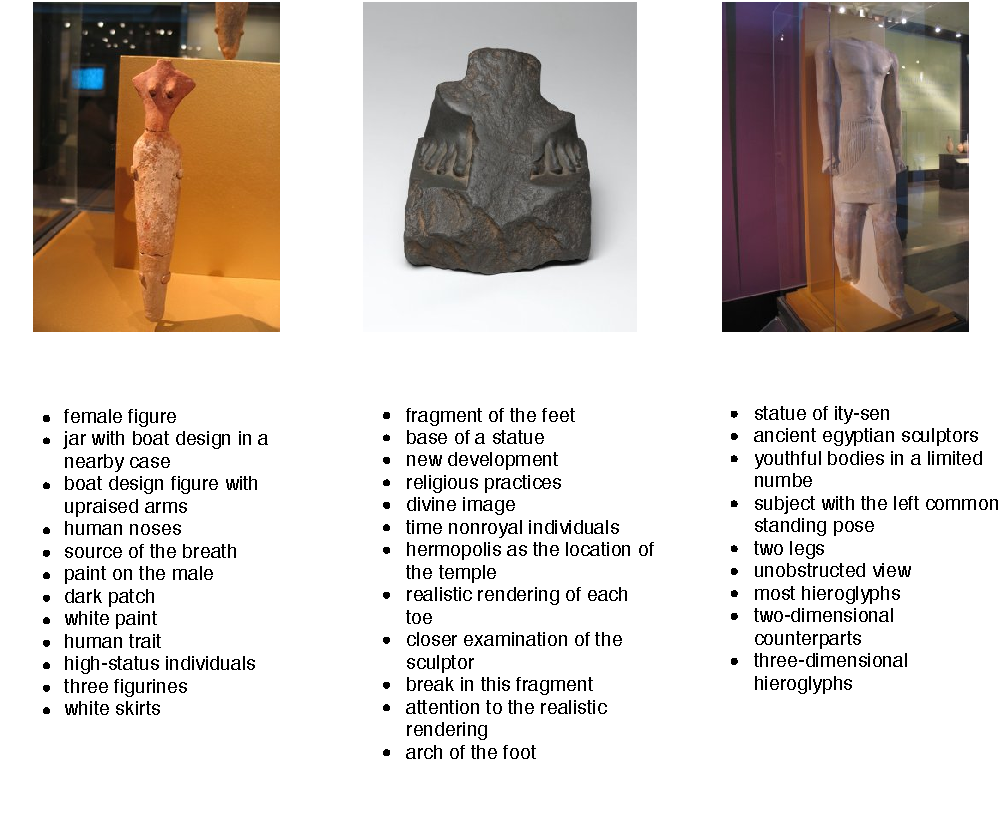
\includegraphics[width=.8\textwidth]{egyptian.pdf}
\caption{Examples of Artworks of Egyptian Artwork Dataset}
\label{fig:sampleEgyptian}
\end{figure}

\begin{figure}[h!]
\centering
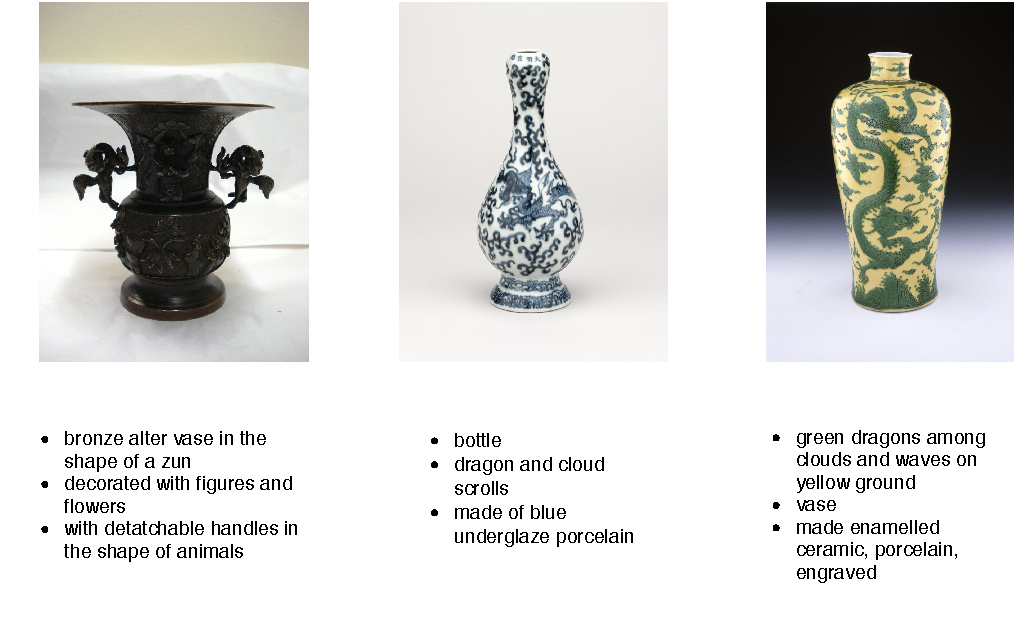
\includegraphics[width=.9\textwidth]{chinese.pdf}
\caption{Examples of Artworks of Chinese Artwork Dataset}
\label{fig:sampleChinese}
\end{figure}

\subsection{Examples of Cross Modal Retrieval under Different Levels}
%% SHURONG: replace the word 'generate' with 'retrieve'. Otherwise it's a bit confusing about what you have done, image captioning or cross modal retrieval. Also replace 'caption' into noun phrases, because the dataset you use are not textual captions any more, they are noun phrase attributes in the images.
In this section, we look at two simple examples of ancient Egyptian artworks and how textual description can be retrieved to match its image under two coarse-grained and fine-grained levels.

\begin{figure}[h!]
\centering
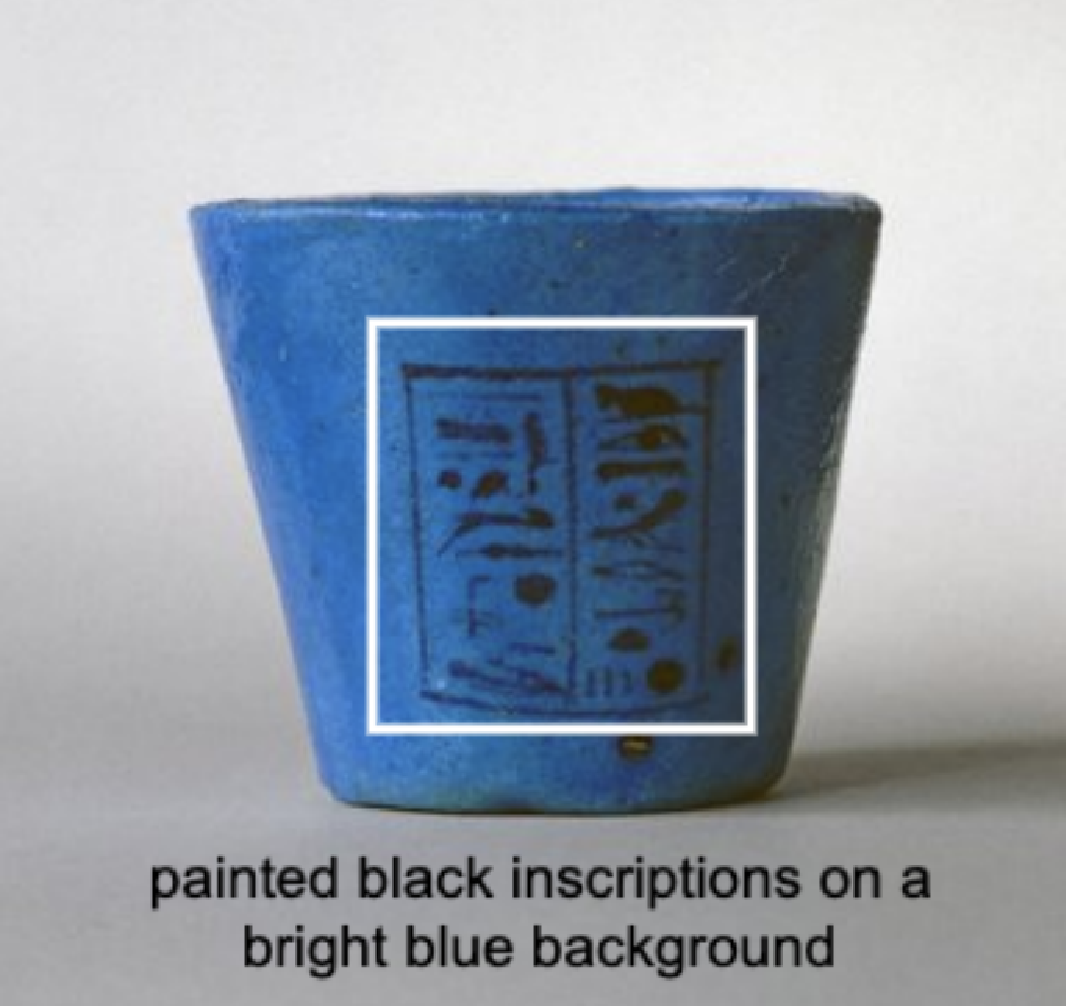
\includegraphics[width=0.4\textwidth]{artwork_fine1.pdf}
\caption{Ancient Egyptian Artwork Example (coarse-grained)}
\label{fig:artwork1}
\end{figure}

%% SHURONG: The examples here are a bit confusing. coarse-grained task target full-image/sentence level retrieval while fine-grained task target fragment-level retrieval (image regions and textual attributes) So according to this defination, the example given in Figure 1.3 is also fine-grained retrieval because the text describes the image content marked by the bounding box. Maybe you can also explain this when you mention these two tasks. Sorry if I didn't explain this clear[done!thx!]
Figure \ref{fig:artwork1} shows a porcelain cup with green pattern on it. Using a coarse-grained multi-modal retrieval model, we can retrieve the textual description sentences ``\textit{Porcelain stem cup with polychrome overglaze enamels}'', which is sufficient for recognising this artwork. However, this retrieved result does not contain more detailed information such as ``\textit{there are two men in independent scenes contemplating the moon in a landscape setting with inverted plantain leaves around the stem and a further figure inside the cup in a red double ring medallion which is much worn}''. 

In the real-world scenarios, there is much more likely for us to encounter an artwork showing in Figure \ref{fig:artwork2}. Our traditional coarse-grained multi-modal retrieval model retrieves ``\textit{a red and a white pot}'' for this artwork but it is not detailed and did not cover sufficient information in the artwork image. Therefore, this motivated us to propose a fine-grained multi-modal retrieval model which can focus on the fragment level image/sentence retrieval. The description on the image was retrieved by our fine-grained multi-modal retrieval model, which has significantly more detailed information.

\begin{figure}[h!]
\centering
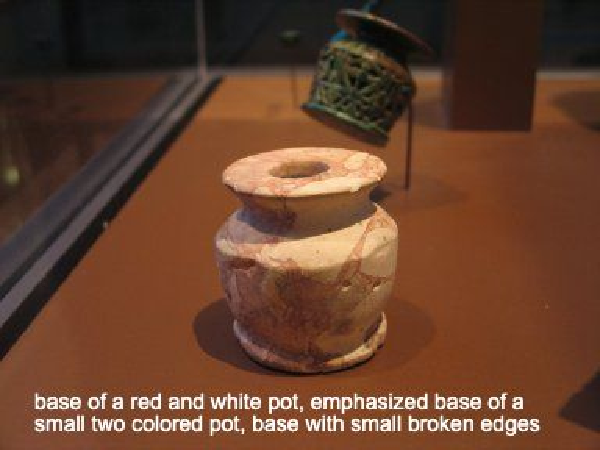
\includegraphics[width=0.5\textwidth]{artwork_fine2.pdf}
\caption{Ancient Egyptian Artwork Example (fine-grained)}
\label{fig:artwork2}
\end{figure}

\section{Research Questions}

In this thesis, we study image-text alignment for artworks in coarse and fine-grained levels. Fine-grained image-text alignment refers to the fragment level cross modal retrieval. The prior sections list the background and motivations, the specific research questions that we look at are:

%% [edited]two research questions: 1. is the alignment model experimented on natural images effective for artwork items 2. can coarse-grained cross-modal retrieval modal be adapted to fine-grained retrieval and how?
\begin{itemize}
    \item Is the image-text alignment model experimented on natural images effective for artwork datasets?
    \item Can coarse-grained cross modal retrieval model be adapted to fine-grained retrieval and how?
\end{itemize}

\subsection{Cross Modal Retrieval Framework}

As mentioned above, our primary research task here is to achieve cross modal retrieval (i.e. between image and text) for artworks. Figure \ref{fig:framework} illustrates a brief working framework for the tasks in a fine-grained level.

%% [solved]shurong: the training data is a bit confusing. an image should be composed of a certain number of image fragments and the text is noun-phrase composed sentence .Or the picture can be kept here but you explain the two levels of retrieval clearly or even give examples.
\begin{figure}[h!]
\centering
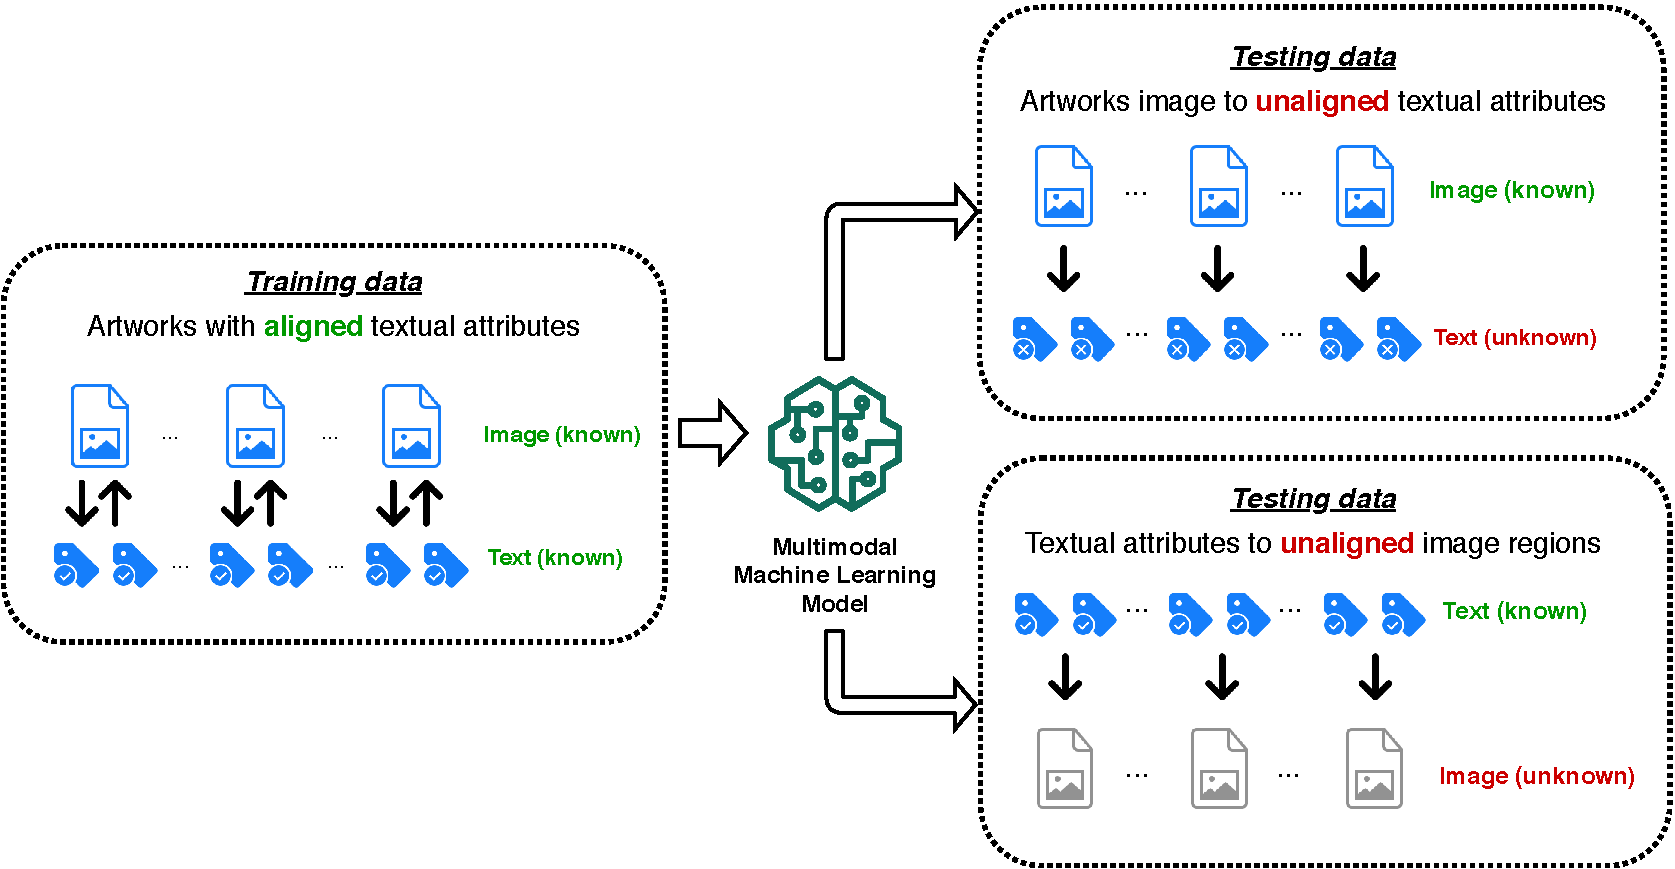
\includegraphics[width=\textwidth]{framework.pdf}
\caption{Cross Modal Retrieval Process (fine-grained)}
\label{fig:framework}
\end{figure}

We train our multi-modal machine learning model on the known image features and corresponding textual attributes; this training process helps us learn the potential relationships between image and text. This trained model will be used to retrieve textual attributes from known image features and vice versa. We believe this may help with automating the artwork annotation process and significantly save labours on manually annotating artwork information.
%% SHURONG: on manually annotate artwork information[done]
%artworks classifications and searches.


\section{Contributions}
The main contributions made by this thesis are:

\begin{enumerate}
    \item We review work from several disciplines which may be of relevance to the present subject of inquiry and provide commentary on how the findings from these disciplines may be useful. (Section~\ref{cha:relatedworks})
    \item We adopted SCAN \cite{scan} as the coarse-grained cross modal retrieval model, analysed its structure and applied it on our proposed Egyptian and Chinese artworks datasets to achieve the image-text alignment. 
    %%SHURONG: The fine-grained model is not an improved task compared with the coarse-grained task. It's better to say that 'this lays the foundation our novel task of fine-grained cross modal retrieval for artwork items'[hearhear]
    By employing this model, we are able to have a coarse-grained alignment between artworks image and textual attributes. This lays the foundation our novel task of fine-grained cross modal retrieval for artwork items. (Section~\ref{cha:scan})
    \item By focusing on fragment level image features and textual attributes instead of feeding the whole images and sentences, we are able to perform cross modal retrieval in a more fine-grained level. This allows the future multi-modal retrieval tasks on artworks to achieve more
    %% SHURONG: I guess you mean more detailed results? Because fine-grained retrieval intends to perform worse than coarse-grained level?[done]
    detailed results. (Section~\ref{cha:Method})
\end{enumerate}


\section{Structure of Thesis}

This thesis is structured into the following chapters:

\begin{itemize}
    
    \item \textit{Chapter~\ref{cha:intro} Introduction}\newline
    We provide the reader with a relevant background to understand this thesis.

    \item \textit{Chapter~\ref{cha:relatedworks} Related Works}\newline
    We introduce relevant research in image recognition, deep learning, object detection, natural language processing and image-text alignment. In particular, we detail seminal research and review the overall state of the current research. We also review the difference in the works pertaining to the traditional visual-semantic alignment technique versus the more recent cross attention image-text alignment framework.
    
    \item \textit{Chapter~\ref{cha:scan} Coarse-grained Cross Modal Retrieval}\newline
    We introduce our coarse-grained cross-modal retrieval modal - SCAN, discuss how its components interact with each other and explain how SCAN uses cross attention to improve image-text alignment. We also show the preliminary result running SCAN on our ancient Egyptian and Chinese artwork datasets.
    
    \item \textit{Chapter~\ref{cha:Method} Fine-grained Cross Modal Retrieval}\newline
    %% SHURONG: likewise, not improve model but a novel task.[done]
    We proposed our novel fine-grained cross modal retrieval model, which now focus more on the fragment level image-text alignment. We then perform several experiments on evaluating the effectiveness of our image generation from text and vice versa by the recall. We also point out the direction of
    possible future improvements by discussing several recent related publications.
    
    \item \textit{Chapter~\ref{cha:conclusion} Conclusion}\newline
    We conclude the work and add some final reflections and remarks.
\end{itemize}
%%% Local Variables: 
%%% mode: latex
%%% TeX-master: "thesis"
%%% End: 
